\documentclass{mproj}
\usepackage{graphicx}
\usepackage{longtable}
\usepackage[backend=biber,
style=trad-abbrv]{biblatex}
\addbibresource{mproj.bib}
\renewcommand*{\bibfont}{\footnotesize}
\usepackage{url}
\usepackage{fancyvrb}
\usepackage{float}
\usepackage[final]{pdfpages}
\usepackage{hyperref}
\hypersetup{
	urlcolor=blue}
\usepackage{fancyhdr}

% for alternative page numbering use the following package
% and see documentation for commands
%\usepackage{fancyheadings}


% other potentially useful packages
%\uspackage{amssymb,amsmath}
%\usepackage{url}
%\usepackage{fancyvrb}
%\usepackage[final]{pdfpages}

\begin{document}
\pagenumbering{roman}

%%%%%%%%%%%%%%%%%%%%%%%%%%%%%%%%%%%%%%%%%%%%%%%%%%%%%%%%%%%%%%%%%%%
\title{A secure client-server mobile chat application implementing an elliptic curve integrated encryption system (ECIES) and other security features.}
\author{Daniel Furnivall}
\date{1st April 2022}
\maketitle
%%%%%%%%%%%%%%%%%%%%%%%%%%%%%%%%%%%%%%%%%%%%%%%%%%%%%%%%%%%%%%%%%%%

%%%%%%%%%%%%%%%%%%%%%%%%%%%%%%%%%%%%%%%%%%%%%%%%%%%%%%%%%%%%%%%%%%%
\begin{abstract}
abstract goes here
\end{abstract}
%%%%%%%%%%%%%%%%%%%%%%%%%%%%%%%%%%%%%%%%%%%%%%%%%%%%%%%%%%%%%%%%%%%

%%%%%%%%%%%%%%%%%%%%%%%%%%%%%%%%%%%%%%%%%%%%%%%%%%%%%%%%%%%%%%%%%%%
\educationalconsent

%%%%%%%%%%%%%%%%%%%%%%%%%%%%%%%%%%%%%%%%%%%%%%%%%%%%%%%%%%%%%%%%%%%

\newpage
%%%%%%%%%%%%%%%%%%%%%%%%%%%%%%%%%%%%%%%%%%%%%%%%%%%%%%%%%%%%%%%%%%%
\section*{Acknowledgements}

I would like to thank my supervisor, Mark McGill for consistently providing suggestions that made me question my own thought process and adjust my approach for the better. The constant support throughout the project is something I am incredibly grateful for.

I would also like to say thanks to Ewa Wanat, Tzvi Lipschitz, Thaïs Ramdani and Matt Weston for deeply helpful stylistic guidance, Bryce Campbell for top tier music recommendations, Conal Brosnan for Kotlin evangelism, Karim Al Tom for Lebanese sweets. Additionally, I'm extremely grateful to Emer Sweeney, Stuart Allan and Michael Callan for their much-needed assistance.

Lastly, I would like to thank my wife Rona and my furry friend Gordon for providing much needed moral support throughout the development and writeup process. 

%%%%%%%%%%%%%%%%%%%%%%%%%%%%%%%%%%%%%%%%%%%%%%%%%%%%%%%%%%%%%%%%%%%
\tableofcontents
%%%%%%%%%%%%%%%%%%%%%%%%%%%%%%%%%%%%%%%%%%%%%%%%%%%%%%%%%%%%%%%%%%%

%%%%%%%%%%%%%%%%%%%%%%%%%%%%%%%%%%%%%%%%%%%%%%%%%%%%%%%%%%%%%%%%%%%

\chapter{Introduction}\label{intro} \setcounter{page}{1} \pagenumbering{arabic}

In an increasingly digital world, we are constantly producing data (and, of course, corresponding metadata). It's estimated that humanity created somewhere in the order of 2.5 exabytes of digital data per day in 2018\cite{baeza2022attention} and the growth of digital data creation by individuals is constantly accelerating.\cite{baeza2022attention} 

As storage costs decrease over time\cite{walter2005kryder}, economic and political incentives have begun to develop for nation state actors and major organisations to develop profiling systems using large-scale data collection and mining. These ``Big Data'' profiling systems are already being used for targeted advertising\cite{farahat2012effective}, market segmentation\cite{pantelis2013understanding}, criminal investigations\cite{zawoad2015digital} and sentencing\cite{simmons2017big}. In the political sphere, these models have been used for increasingly effective traditional campaigning, \cite{kreiss2019arbiters} as well as (alleged) mass psychological manipulation\cite{berghel2018malice} and disinformation\cite{stocker2019facebook} campaigns.

The question of whether the average individual is able to enjoy the fruits of such data collection is less clear. Do these large actors have the best interests of the subjects of their data in mind? If not, methods for obfuscating or hiding sensitive data become valuable considerations.

In a pre-digital world, an individual could avoid eavesdropping or data collection by malicious entities by simply speaking in a hushed voice, shredding documents, moving quietly or looking over their shoulder. In the current landscape, it is much more difficult to avoid surveillance without eschewing technology entirely. Our mobile phones are constantly communicating our triangulated locations, and even if our web traffic is encrypted by default, browser or ISP metadata still contains useful profiling information.

Secure messaging applications aim to allow individuals to communicate with other individuals around the globe while avoiding the potential for eavesdropping. In theory, this means the user can enjoy the benefits of a globally connected world while preserving their own privacy. However, in practice there are of course many implementation challenges to be considered.

\section{Why are secure chat applications needed?}
Secure messaging applications provide a means of communication between individuals or groups across a network of some kind. This can take the form of text, audio or video messaging, document or file sharing.

To begin to understand the users of secure chat applications, two important questions need to be answered:
\begin{enumerate}
	\item Who desires secure messaging?
	\item Who are they aiming to protect their data from?
\end{enumerate}

There are many categories of potential users of such applications, and from wildly different settings. These can be mundane and innocuous, such as the organisation of a surprise party for a friend or family member. 

However, another group of potential users are those who seek to hide criminal behaviour from law enforcement organisations. A high-profile example of this would be the EncroChat network of encrypted phones, predominantly used by organised crime, which was unveiled after a Europe-wide infiltration and investigation of the network by law enforcement groups (leading to several thousand arrests) \cite{sommer2022evidence}. 

Another group who may wish to evade police or law enforcement are political dissidents. In what has become known as the "Million Dollar Dissident" \cite{marczak2018hide} case, a dissident in the UAE, Ahmed Mansoor, was targeted by the NSO group (an Israeli cybersecurity firm which produces spyware for government use). He subsequently had his passport confiscated, he was beaten multiple times, his car was stolen and finally he was imprisoned by the UAE authorities - all within a week of posting anti-government posts online \cite{mazzetti2019new}. There are many parallels here with other groups who benefit from secure messaging - whistleblowers sharing information with journalists, and police informants who need to share data secretly with law enforcement. 

In reality, there are plenty of reasons for \emph{everyone} to use secure messaging such as protecting data in case of device theft, avoiding embarrassment, or limiting exposure to blackmail or government surveillance. Continuing the comparison to real-world communication - when speaking out loud, people don't tend to shout all the time, and tend to consciously limit and monitor who is listening to a conversation.

It should be clear that although there are many categories of potential secure messaging users, there are also many potential adversaries for these kinds of platforms, which means the development of such services is a complex undertaking. There are major tradeoffs which need to be made between usability and data security - for example, how can we preserve security of messages while also storing them on a mobile device? 

\section{Objectives}
The primary development objective of this project was to develop an Android mobile application (and corresponding server) that uses complex security features including an end-to-end encryption solution that uses both asymmetric (Elliptic Curve Diffie-Hellman) and symmetric (AES) encryption approaches, pseudonymous identity and self-destructing messages. 

During the development journey of this application, the intrinsic motivation was to come to a greater understanding of the complexities, assumptions and tradeoffs involved in creating these kinds of platforms. 

\chapter{Requirements and \\ Analysis}\label{analysis}
Unger et al's ``Systematization of Knowledge'' (SoK) 2015 paper on secure messaging captured in extensive detail some of the key considerations for developing secure messaging applications. They highlighted three points which comprise the major challenges in this field - trust establishment, conversation security and transport privacy.

Trust establishment describes the problem of ensuring that users are communicating with the party they intended. This is a difficult problem, as there are tradeoffs between security and usability that need to be made. One method which has seen extensive use is key-sharing. This ensures that the recipient of a message is able to verify that it was sent by the sender.

Conversation security in this context refers to the security protocol used to encrypt the data. Unger et al lament the fact that most secure messaging solutions use only static asymmetric encryption (i.e. long-term key persistence meaning users do not need to exchange keys regularly). This is another example of the usability/security tradeoffs that need to be made for wider adoption of secure messaging.

The final challenge is transport privacy, which concerns how messages are transmitted between users. This is a complex problem, as metadata such as the identity of the sender and recipient need to exist so that the server can route messages correctly, despite also being appealing attack vectors for malicious actors.

\section{Existing applications in this field}
There are many existing secure chat applications available for both iOS and Android, with wild variation in terms of encryption architecture, as well as other security and usability features. For brevity, this brief review focuses on the three largest mobile secure messaging providers in 2022 - Signal, Telegram and Whatsapp.

The table below highlights some of the features and attributes of each of these applications:

\makebox[\linewidth]{
\begin{tabular}{|p{2.5cm}|p{3.8cm}|p{3.8cm}|p{3.8cm}|}
		\hline
	Application & Signal & Whatsapp & Telegram \\
	\hline
	Ownership & Signal Foundation (non-profit, USA) & Facebook Corporation (USA) & Durov Brothers (Russian) \\
	\hline
	End-to-end Encryption & Double Ratchet Algorithm\cite{alwen2019double}, constantly cycling symmetric session keys and Elliptic Curve Diffie-Hellman (ECDH) keypairs - this approach is called the ``Signal Protocol'' & Proprietary implementation of the Signal Protocol (unverifiable). Does not apply to backed-up messages stored on Google servers. & Only available in ``Secret Chats'', and only on mobile devices - uses Telegram's own MTProto 2.0 protocol\cite{jakobsen2016cca}. For group chats, messages are encrypted symmetrically and are theoretically readable by the server.\\
	\hline
	Open Source & Fully open source for both client and server (with the exception of a server-side anti-spam component) & Entire closed source & Open source client with a closed source server.\\
	\hline
	Self-destructing messages & Controlled by the sender (i.e. the messages will be deleted from the recipients device based on the sender's settings). Manageable via defaults or for individual conversations. Timespan variable. & Sender-controlled, can be managed individually or via defaults. Fixed timeframe of 7 days. & Sender-controlled, can be managed individually or via defaults. Timespan variable.\\
	\hline
	Group chats & Fully E2EE encrypted using ``client-side fanout''\cite{jansen2020security}, where each message is encrypted individually to all users in the group. & Same as Signal (unverifiable due to closed source) & Encrypted between client and server but not E2EE.\\
	\hline
	Pseudonymous Messaging & Not available (linked to phone number) & Not available (linked to phone number) & Not available (linked to phone number, although it is possible to hide phone number from contacts after creation.)\\ 	
	\hline
	Metadata collection & Only stores phone number used to register, date of initial registration and date of last app use. & Historical message metadata, phone contacts, device metadata and activity, blocked numbers, read receipts, full name and more. & IP addresses, phone contacts, historical message metadata.\\ 
	\hline
\end{tabular}
}

\section{Issues in existing applications}
As can be seen in the table, Signal appears to be the most secure of the available secure messaging applications. This comes from a combination of best-in-class encryption, open source code allowing for security audits, fine-grained control of privacy options and innovative handling of security such as their use of client-side fanout for group chats. Whatsapp and Telegram both closely guard some or all of their source code, making it impossible for independent researchers to verify that their security claims are accurate. Signal also seems to have limited financial or political incentive to store metadata about the behaviour of their users due to their non-profit ownership model, which contrasts with Whatsapp's ownership by an advertising company and Telegram's \href{https://promote.telegram.org/}{use of advertising via sponsored messages}.

All three applications provide fairly strong capabilities for self-destructing messages. Importantly, all three allow the sender to define the parameters for deletion, although Whatsapp does not provide timeframe granularity compared to Signal and Telegram. This means that users can feel relatively secure in the knowledge that even if the recipient is compromised their own exposure is limited.

One of the major downsides of all three applications is the lack of pseudonymous messaging. This is an understandable omission due to implicit need for chat applications to incorporate some means of social network discovery (in all cases, phone numbers and contact lists are used for this function). 

This means that the development of an application that provides comprehensive end-to-end encryption and self-destructing messages alongside pseudonymous messaging features is worth pursuing.

\section{User Personas}

\emph{Thaïs} - a 37-year-old police informant deeply nested within a major international drug distribution network. She needs to communicate with her handlers within law enforcement securely without arousing the suspicion of her colleagues within the criminal organisation. One of the most important factors in her choice of messaging applications is self-destructing messages. This means that even if her device is compromised, there will be no evidence that she has been sharing information with police.

\emph{Ewa} - a 28 year old human rights activist and political dissident in a large authoritarian state in South-East Asia. As an important agent for change within the country, she needs to alert the country's overseas diaspora, human rights organisations and international media to a new and bloody crackdown on freedom of expression that occurred. The ruling party of the country has implemented state of the art surveillance technology and deep packet inspection on all outgoing web traffic. Ewa needs a means of communicating securely with her intended recipients via an insecure channel. 

\emph{Tzvi} - a 45 year old political ``fixer'' working within the ruling party of a large African state. He has been tasked with giving a veneer of legitimacy to the process of allocating government contracts to political allies through a fraudulent tendering process. This requires him to have a secure communication channel with the chosen contractor so they can ensure they are able to make the most competitive bid. Tzvi has his own political ambitions which could be tarnished by such dealings, making it vitally important for him to have plausible deniability. Using a pseudonymous identity for messaging is a key selling point for him.

\section{Requirements}
Requirements for this application were gathered after a detailed analysis of the existing products in this space. All the features in the application are present in some sense in some or all of the competitor applications analysed with the exception of pseudonymous messaging. Combining several key features (Self-destructing messages, a combination of symmetric and asymmetric encryption and pseudonymous messaging) formed the basis for the design. 

Requirements were then outlined following the MoSCoW requirement prioritisation framework\cite{haughey2011moscow}. This method allows for prioritisation based on four priority levels: 
\begin{enumerate}
	\item ``Must have'' - the most basic requirements to have a functioning solution for the problem. 
	\item ``Should have'' - Requirements that the app should include, but does not absolutely need.
	\item ``Could have'' - Requirements that could potentially be implemented.
	\item ``Would like to have'' - Features which would be nice to include but are not strictly necessary or required.
\end{enumerate}

\subsection{MoSCoW table}
\begin{longtable}{|p{2.5cm}|p{11cm}|}
	\hline
	Prioritisation & Requirement\\
	\hline
	Must have & User can connect to the server application via a client application.\\
	\hline
	Must have & User can send a message from one client to another client.\\
	\hline
	Must have & User can receive a message from another client.\\
	\hline
	Must have & User can create a pseudonymous username.\\
	\hline
	Must have & User identity can persist upon disconnect/reconnection events\\
	\hline
	Must have & User can see other connected users within a contacts page\\
	\hline
	Must have & Messages (sent and received) are stored locally on the client within a local database.\\
	\hline
	Must have & User can talk to more than one user independently in separate messaging sessions.\\
	\hline
	Must have & User messages reach the correct recipient only.\\
	\hline
	Should have & User can send encrypted messages which cannot be read by the server operator.\\
	\hline
	Should have & User is able to define how long to store messages in the local database.\\
	\hline
	Should have & User receives a push notification when a message is received.\\
	\hline
	Should have & User preferences (e.g. self-destruct preferences) should persist on application restart \\
	\hline
	Should have & Recipient public keys should be shared with sender as appropriate.\\
	\hline
	Should have & Private/Public keypairs should be stored securely to prevent unwanted access.\\
	\hline
	Should have & Generating keypairs should be fast while also secure.\\
	\hline
	Could have & Group messaging between multiple users.\\
	\hline
	Could have & Users can access the application via a web-based interface in addition to the mobile application.\\
	\hline
	Could have & Users can format their text using standard decorations (e.g. bold/italics/strikethrough)\\
	\hline
	Could have & Users can forward messages from one user to another user.\\
	\hline
	Would like to have & Message queueing to allow users to receive messages when they reconnect.\\
	\hline
	Would like to have & Sender-defined self-destructing messages.\\
	\hline
	Would like to have & E2EE on group chats using client side fan-out method.\\
	\hline
	Would like to have & Users can record audio messages and transmit to another user.\\
	\hline
\end{longtable}

\section{User stories}
User stories are a means to map requirements to actionable feature development and separate workload into manageable chunks and a key tenet of Agile methodology. Indeed, a 2018 study found that approximately 90\% of Agile practitioners utilised user stories in their requirements gathering process\cite{dalpiaz2018agile}.
The user stories below represent the desired behaviours from the application and were used as a framework for developing the application in an agile framework.
\begin{itemize}
	\item As a user, I want to be able to send messages from my client application to the server for handling.
	\item As a user, I want my message to be routed to the appropriate client device of my choosing.
	\item As a user, I want to create a pseudonymous username which is shown to other users.
	\item As a user, I want to view other connected users.
	\item As a user, I want messages on my device to disappear after a given time period
	\item As a user, I want to encrypt my messages so that the server cannot read the contents.
	\item As a user, I want to be able to decrypt messages that are transmitted to me from the server.
	\item As a user, I want my data (e.g. username) to persist after I close the application.
	\item As a user, I want to receive a push notification when a message is sent to my device if I am doing something else.
	\item As a user, I want to be able to click on a notification and be taken directly to the relevant chat window to reply to the sender.
	\item As a user, I want the contacts list to automatically update when a user connects or disconnects from the server.
	\item As the server operator, I do not want to be able to read the content of messages sent to me.
	\item As the server operator, I want to be able to update stored client public keys when they are changed.
\end{itemize}

The above stories formed the basis for the development process, the intricacies of which are discussed extensively in the following chapter.

\chapter{Design and \\ Implementation}\label{design}
\section{High Level Architecture}
Some of the primary architectural considerations on this project are highlighted below:
\begin{enumerate}
	\item Client-side encryption to allow messages to flow through the (untrusted) server.
	\item Client-side self-destructing messages according to client-defined storage duration parameter.
	\item Persistence of user identity and handling of disconnection/reconnection events.
\end{enumerate}
The figure below represents a very high level view of the system architecture, which gives an overarching perspective of how the system fits together and some of the technological choices made. However, it does not give a comprehensive picture of the complexity of the overall system.

\begin{figure}[h!]
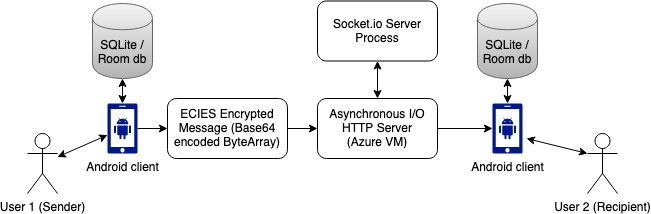
\includegraphics[scale=0.5]{images/high-level-architecture.png}
\caption{High level architecture of the system}
\end{figure}

\section{WebSockets vs REST API}
One of the major decisions required for this project was which transport protocol to use for propagating messages through the system. The two major options considered were a REST API via HTTP\cite{masse2011rest} and WebSockets\cite{fette2011websocket}. 

REST (Representational State Transfer) is a set of design principles which assists in the development of web services which utilise a central server with one or many clients, based on the twin concepts of request and response. A client will send a request to a server and receive a response based on the content of the request. REST APIs are heavily used across many industries and mostly (though not exclusively) use the HTTP protocol to communicate between client and server. The primary weakness of REST is that it is not optimal for circumstances where constant bi-directional communication is important between client and server. Indeed, the WebSocket Protocol Standards Track Document\cite{fette2011websocket} states the problem as such:

\begin{verbatim}
Historically, creating web applications that need 
bidirectional communication between a client and a server 
(e.g. instant messaging and gaming applications) has required 
an abuse of HTTP to poll the server for updates while
sending upstream notifications as distinct HTTP calls.
\end{verbatim}

The WebSocket protocol is a newer system which excels in two-way communication between client and server systems. For chat applications like the subject of this project, WebSocket appears perfectly suited to the problem.
Due to the comparative simplicity of bidirectional communication using WebSockets, the protocol uses significantly less energy\cite{herwig2015assessment} to maintain a client/server connection. This is especially relevant when considering that this is a mobile application which needs to preserve battery life. 
The one major downside of WebSockets is that it is a modern standard which is not necessarily fully supported across all devices or browsers yet.

During the literature review of this topic, it became apparent that there was a way to achieve the best of both worlds. Socket.io\cite{rai2013socket} is a cross-platform library which initially attempts to create a WebSocket connection and, if not possible, falls back to HTTP polling for devices which do not support it. It also provides helpful additional features like automatic reconnection. It was determined that both client and server implementations existed in the desired languages (Python/Kotlin) and subsequently included in the system design.

\section{Encryption Implementation}\label{encryption}
As mentioned previously, the system was designed with the prevailing goal of having two clients who could communicate with each other through an insecure, untrusted environment (i.e. the server) without needing to worry about messages being vulnerable to man-in-the-middle attacks\cite{mallik2019man}. The most attractive means of achieving this is to use state of the art encryption.

An oft-repeated adage in secure software development is that a developer should "Never roll your own crypto"\cite{apvrille2005secure}. This is due to the fact that encryption is almost always absolutely critical to the functioning of applications. Furthermore, it is very easy for a developer's code to provide the illusion of working security features without fully understanding possible attack vectors. As such, all cryptography utilised in this project has an extensive track record of use in commercial and governmental settings.

Two of the most prevalent encryption approaches used in the modern world are asymmetric and symmetric encryption. Symmetric encryption is the simpler of the two - a secret key is used to alter the content of a piece of plain text in such a way that it's unreadable to anyone except someone who also has the secret key and can use it to decrypt the message. The major flaw with symmetric encryption is the need to share the secret key with the recipient. If the recipient does not have access to the secret key, they cannot decrypt the message. Similarly, if the secret key is intercepted during transport of the message, a bad actor can decrypt the message. A good example of the symmetric encryption approach is the Advanced Encryption Standard (AES), which is used in this project. The AES algorithm was designed by Vincent Rijmen and Joan Daemen in 1999 and defined as a standard by the United States Government in 2001.

Asymmetric encryption is a little more complex - a key pair consisting of a public and a private key, which are separate but mathematically linked is used to encrypt and decrypt data. To send an encrypted message to the intended recipient, the sender must use their own private key and the recipient's public key. The recipient can then use their own private key and the sender's public key to decrypt the message at the other side. The primary issue with asymmetric encryption is that it's significantly more complex to implement than symmetric alternatives, and key generation is slower.

Two of the most common types of asymmetric encryption are the Rivest Shamir Adleman (RSA) algorithm\cite{rivest2019method} and Elliptic Curve Cryptography (ECC)\cite{lopez2000overview}. The RSA algorithm has been in use for 45 years, and utilises the factorisation of prime numbers to produce a unique keypair. ECC is a more modern algorithm which uses the structure of elliptic curves to generate keypairs. The primary advantage of ECC over RSA is the computational requirements to generate unique keys - as the key size required for secure communication increases (i.e. when malicious actors are able to use greater computational power), the key generation process becomes prohibitively expensive. In a 2015 study, an Indian team found that RSA keypair generation was 471 times slower than the equivalent ECC keypair process when keys reached a certain size\cite{gobi2015comparative}.

The approach taken on this project was to use a combination of both asymmetric and symmetric approaches - this combination means that the comparative speed of symmetric approaches can be harnessed for converting the plaintext to ciphertext, and the additional security provided by asymmetric encryption, ensuring that only the intended recipient can open the message as the symmetric key is independently generated by both sender and receiver from a shared secret.The implementation used is known as an Elliptic Curve Integrated Encryption Scheme (ECIES)\cite{martinez2010comparison}. ECIES is a hybrid encryption system which was devised by Victor Shoup in 2001. It comprises of three key functions:
\begin{enumerate}
	\item A key agreement function to generate ``shared secrets'' from a user's public key and another user's private key.
	\item A key derivation function which is able to produce a key from an input of some kind.
	\item A symmetric encryption algorithm which is used with the shared secret as a key to encrypt the plain text.
\end{enumerate}
The advantage of ECIES is that it provides very strong encryption for secure communication within an untrusted/insecure channel while also having desirable properties for mobile devices such as much smaller keys than similar asymmetric/symmetric hybrid approaches (as shown by Martinez et al when comparing to RSA/AES hybrid systems\cite{martinezECIES})

The ECIES implementation used in this project uses the following algorithms and approaches:
\begin{itemize}
	\item Elliptic Curve Diffie-Hellman\cite{maurer2000diffie} to generate a shared secret over an untrusted channel. 
	\item The P-521 elliptic curve outlined by the National Institute of Standards and Technology (NIST)\cite{brown2001software}
	\item The SHA-512 cryptographically secure hashing function, of which the first 32 bytes are used to generate the AES key for the key derivation function.
	\item AES-256 for the symmetric component, generated from the shared secret.
\end{itemize}

\section{Self-destructing Messages}
One of the features implemented in the application is self-destructing messages on a client device. This allows the user to define a duration to store received and sent messages on their device, after which the specific message is deleted. This feature was implemented by prompting the user on their first time starting the application to define a duration for message storage which is passed as a parameter to a daemon process (a background thread which runs at very low priority) which sends a parametrised SQL query to the database, deleting message objects based on their timestamp metadata. Discussion of how this duration is persisted after restarts can be found in the following section.

\section{Persistence of users after disconnects}
One of the most complex challenges faced during the development of the application was persisting clients after they disconnect and reconnect from the server. This was handled in the following manner:
\begin{figure}[H]
	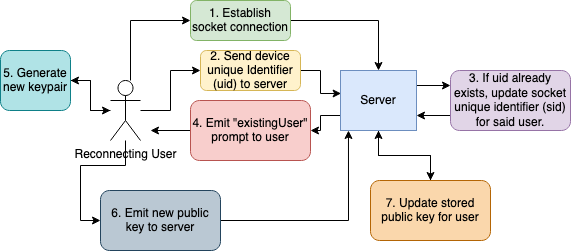
\includegraphics[scale=0.6]{images/reconnection-flow.png}
	\caption{Reconnection flow for user persistence}
\end{figure}
The complexity of this process comes down to an inherent limitation of Android's built-in cryptography libraries. The system design was predicated on the assumption that it would be possible to securely store public and private keys within the Android KeyStore\cite{cooijmans2014analysis}, a secure storage system within Android which is capable of storing public and private keys. However, the KeyStore does not currently support Elliptic Curve keypairs, which meant that the design had to be altered to accomodate this. What this means in practice is that a new keypair is generated on reconnection - the private key is stored locally and the public key is emitted to the server which replaces the existing stored key. 

The flexibility to easily generate new keypairs is a huge advantage of elliptic curve cryptography - the key generation process is so quick that it's imperceptible to the user - something that would not be possible with RSA encryption.

\subsection{Storage of self-destruct duration}
Although there is no secure key-value store that allowed for the storage of ECDH keypairs, there is a non-secure method for persistence of key-value data (not including the database) using ``SharedPreferences'' files. These are ideal for storing configuration properties which persist after closing the application. This means that the initial value prompted from the user to request self-destruct message duration is able to be persisted and a returning user will be able to maintain their configuration, while also maintaining separation of concerns and reducing excessive exposure to database operations.

\section{Message Propagation}
The figure below describes the entire journey of a message through the messaging system. The colour scheme for the various key stages is broadly represented by the following:
\begin{enumerate}
	\item Green: Initial message composition, server querying and local storage.
	\item Yellow: Asymmetric + symmetric encryption, encoding and send process
	\item Red: Server routing for message
	\item Purple: Receipt, decryption, display and storage of message.
\end{enumerate}

\begin{figure}[H]
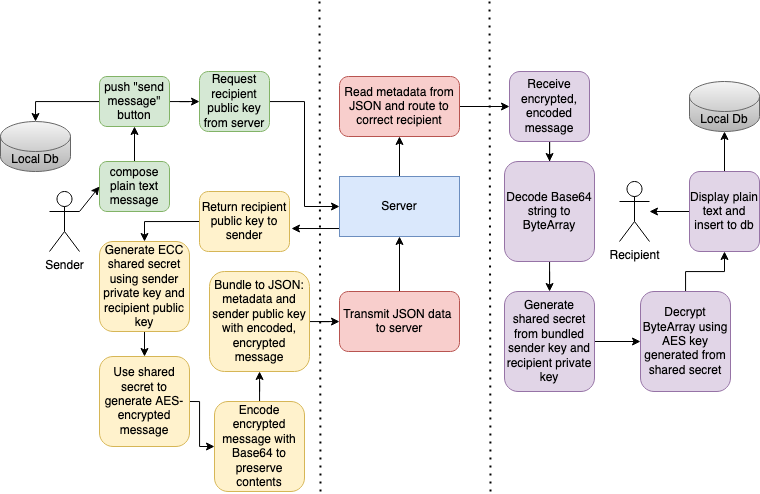
\includegraphics[scale=0.5]{images/message-flow.png}
\caption{Flowchart of the journey of a message from one client to another}
\end{figure}

\section{Design Patterns}
During the development of this project, a concerted effort was made to follow established design patterns and best practice wherever possible. It is a testament to the design of the Android development environment and documentation that this was relatively trivial to achieve. 

In addition, wherever possible, adherence to the ``Don't repeat yourself'' (DRY)\cite{10.5555/320326}, ``Keep it simple, stupid'' (KISS), and five SOLID principles\cite{martin2000design} was paramount.

The table below shows the design patterns which were deliberately utilised in the development of this project:
\begin{center}
\begin{tabular}{ |p{4cm}|p{4.5cm}|p{5.0cm}|}
	\hline
	Pattern & Concise Definition & Implementation\\
	\hline
	Command Pattern\cite{sarcar2020command} & Encapsulation of a request into an object  & Socket.io event handler objects in both client and server\\
	\hline
	Observer Pattern\cite{eales2005observer} & When one object changes state, dependents update accordingly & LiveData queries updating views as events occur (ChatWindow and Contacts)\\
	\hline
	Adapter Pattern\cite{harmes2008adapter} & Allow an interface of one class to be used as another interface & ContactsAdapter for RecyclerView and MessageListAdapter for displaying chat messages.\\
	\hline
	Builder Pattern\cite{sarcar2016builder} & Simplifies object creation step-by-step & Push notification builder object allows for customisable notifications.\\
	\hline
	DAO Pattern\cite{long2004data} & Data Access Objects provide abstract interface for database, separating low level and high level operations & ChatMessageDAO allows us to specify the exact queries we can use on the database and prevents any other type of unplanned operations.\\
	\hline
	Singleton Pattern\cite{stencel2008implementation} & Restrict instantiation of class to exactly one instance & SocketHandler.kt in the client is an example of a class which should be (and is) a singleton.\\
	\hline
\end{tabular}
\end{center}
It is also worth mentioning that the Model-View-Viewmodel architectural style was adopted throughout the application, as it is the recommended architectural pattern recommended by the Android core development team\cite{androiddevelopers}. 
This architectural style is most clearly seen in all interactions between the database, the repository, the data access object and the ViewModel which displays data in the ChatWindow.kt activity.

\section{User Interface and Visual Design}
User interface was not a primary concern for the application, but during the requirements process, Balsamiq was used to design simple mockups of the application. These mockups do not reflect the final state of the application but they are included in the appendices for posterity.

Future development of the application will in part focus on improving the visual design.


\section{Development tooling}
There are two primary components to the overall system - one or more Android mobile client applications which communicate with a central, deployed server.


\subsection{Client}
The final client application was written entirely in the Kotlin language (v1.6.10) using the Android Studio IDE. 

\subsubsection{Development and debugging process}
Traditional Android software development involves using the qEmu device emulator built into Android Studio to imitate the experience of a real user on their own device. 

Debugging code during the HushChat development process was a complex endeavour, as the development machine had fairly limited RAM. As the purpose of the application was communication between two clients, it was important to be able to emulate two devices at the same time so messages could be exchanged. This was initially possible on the development machine, but became unfeasible over time as the complexity of the system grew and memory capacity became constrained. 

The debugging environment eventually morphed into a single qEmu emulated device on the development machine combined with a physical android device (Google Pixel 4). This methodology became possible with the introduction of Android version 11 and Android Studio `Bumblebee' (v2021.1), which allows the developer to run Android debugging tools (i.e the Android Debug Bridge, or ADB) via WiFi connection. This feature was extremely helpful in the development process, and it allowed for the introduction of further feature complexity that would not have been possible otherwise due to the technical limitations of the development machine. 

Running a WebSocket-based application locally also presented a minor challenge, as qEmu virtual devices use the traditional localhost/127.0.0.1 address to represent their own internal loopback interface rather than that of the host development machine. This meant that to communicate with the locally hosted server, the \href{https://developer.android.com/studio/run/emulator-networking.html}{special debugging address 10.0.2.2 was used.} After the development of the server side of the application was complete, this problem was solved by deploying the server to a static IP address (via a Azure Virtual Machine).

\subsubsection{Key Dependencies}
\begin{itemize}
	\item \href{https://github.com/socketio/socket.io-client-java}{Socket.io} - v2.0.0 - the developers of socket.io provide a native Java implementation. Due to Java's seamless interoperability with Kotlin, this did not cause any implementation problems with the version implemented.
	\item \href{https://www.bouncycastle.org/}{BouncyCastle} - v1.67 - BouncyCastle is the cryptography API that performs a lot of the cryptographic operations within the application, including generation of elliptic curve keypairs. There is a built-in version of BouncyCastle within the Android SDK, but this does not support ECC, which meant that the client application needed to replace the inbuilt library with a more updated version. This can be seen within the codebase with the following calls within the MainActivity and ChatWindow classes:
		\begin{verbatim}
		Security.removeProvider("BC")
		Security.addProvider(BouncyCastleProvider())
		\end{verbatim}
	\item \href{https://developer.android.com/jetpack/androidx/releases/room}{Room ORM} - v2.4.0 - Room provides an object-relational mapping (ORM) over the SQLite database built into the Android SDK. When developing the application, the main data model to consider on the client side was that of an individual chat message, including metadata (e.g. recipient) and content. Working with Room allowed for a more streamlined development experience and reduction of boilerplate code, as it meant working directly with Kotlin (Java) entities instead of writing complex queries for inserting messages to our viewmodel. Traditional SQL queries were still used to capture relevant data to display to the user in chat windows. 
\end{itemize}

\subsection{Server}
The server application was written in Python v3.9.1 in the PyCharm IDE and utilised several libraries which are highlighted below. 

\subsubsection{Key Dependencies}
\begin{itemize}
	\item \href{https://python-socketio.readthedocs.io/en/latest/index.html}{python-socketio} - v5.5.0 - a Python server implementation of socket.io, funded by the original socket.io developers.
	\item \href{https://docs.aiohttp.org/en/stable/}{aiohttp} - v3.8.1 - an asynchronous http server which (importantly) supports websockets. The socket.io process attaches itself to the aiohttp server which allows information to be transmitted and received from clients.
\end{itemize}

\subsubsection{Deployment}
To allow users to message other users, it was necessary to deploy the server application on a static IP address. To do this, a 1GB/1CPU Virtual Machine instance was used, running Ubuntu 20.04 in the West Europe region of the Microsoft Azure cloud platform. 

\subsection{Final report}
This dissertation was written entirely in LaTeX using Neovim v0.5.1 with the VimTex plugin and the Skim PDF reader (which auto-refreshes at compile time). 

\subsection{Version Control}
Git was the version control solution used throughout the project. Mild discomfort with the idea of storing the written report with a private company (Overleaf) while writing meant that it was worth taking the step of compiling the document locally. This had the fortunate benefit of meaning the entire project could be stored in a single git repository (as well as an opportunity to learn a lot of new things). 

The host of choice for the upstream repository on this project was GitHub, and the entirety of the project can be found at the following link. It is important to note that the commenting approach may appear excessive (and does not follow the ``Code tells you how, Comments tell you why'' commenting practice) but this was done with the intention of assisting the reader to get through the code as quickly as possible.  

\href{https://github.com/furnivall/SEng_Final_Project}{https://github.com/furnivall/SEng\_Final\_Project}

%%%%%%%%%%%%%%%%%%%%%%%%%%%%%%%%%%%%%%%%%%%%%%%%%%%%%%%%%%%%%%%%%%%
\chapter{Evaluation \& Testing}\label{testing}
\section{User evaluations}
\subsection{Methodology}
\subsection{Demographics}
\subsection{Issues highlighted}
%%%%%%%%%%%%%%%%%%%%%%%%%%%%%%%%%%%%%%%%%%%%%%%%%%%%%%%%%%%%%%%%%%%
\chapter{Conclusion}\label{conclusion}
\appendix % first appendix
%%%%%%%%%%%%%%%%%%%%%%%%%%%%%%%%%%%%%%%%%%%%%%%%%%%%%%%%%%%%%%%%%%%
\chapter{First appendix}

\section{Section of first appendix}

%%%%%%%%%%%%%%%%%%%%%%%%%%%%%%%%%%%%%%%%%%%%%%%%%%%%%%%%%%%%%%%%%%%
\chapter{Second appendix}

%%%%%%%%%%%%%%%%%%%%%%%%%%%%%%%%%%%%%%%%%%%%%%%%%%%%%%%%%%%%%%%%%%%
% it is fine to change the bibliography style if you want
\printbibliography
\end{document}
